\chapter{Introduction}
\label{chap:intro}

\nomenclature{CPS}{Cyber-Physical System}
\nomenclature{IoT}{Internet of Things}
\nomenclature{ZB}{Zettabytes}
\nomenclature{NLP}{Natural-Language Processing}

Cyber-Physical Systems (CPSs) are a nomenclature created to describe the applications that combine digital aspects with real-world applications. This integration happens through an integrated loop using sensors to add perception and often actuators to interact with the environment \cite{zanero2017cyber}. Some of the essential aspects that enable the development of such systems are hardware miniaturization and the increased number of devices with networking abilities \cite{alguliyev2018cyber}.

Cyber-physical systems relate to some aspects of computer science, especially within the context of embedded computing and edge computing. Among these aspects, we highlight the following related context \cite{alguliyev2018cyber, baheti2011cyber}:

\begin{itemize}
    \item Industry 4.0;
    \item Internet of Things (IoT);
    \item Big data;
    \item Cloud computing;
    \item Edge computing;
    \item Wearable devices;
    \item Mobile devices;
    \item Real-time systems;
\end{itemize}

Our understanding is that these concepts are linked through two fundamental features of cyber-physical systems. The first important concept we raise is the \textbf{context awareness}. Applications of CPSs must have means to perceive the context around them. Then, the second context is \textbf{environmental interaction}. These applications must be able to interact with the users, stakeholders, and the surrounding environment. Besides these main concepts, some of the features from CPSs are \cite{shi2011survey}:

\begin{itemize}
    \item Closely integrated systems;
    \item Resource constrained;
    \item Networked;
    \item Executes in closed loops;
    \item Reliable and secure.
\end{itemize}

Modeling CPSs is a challenge \cite{derler2011modeling}. Applications within this range must integrate system specifications, considering physical restraints, hardware and software integration, and the network interconnecting the devices. Also, software development in CPSs must consider its correctness and often timing constraints.

In this text, we will henceforth name the applications built within the CPS range as cyber-physical applications. Some examples of stakeholders from cyber-physical applications are smart cities, industries, aviation, environmental monitoring agencies and researchers, healthcare professionals and patients, and meteorologists \cite{alguliyev2018cyber, baheti2011cyber, zanero2017cyber, haque2014review}.

As stated before, wearable computing and edge computing are essential concepts within the range of CPSs. In this work, we explore how to use both these concepts together with artificial intelligence algorithms to create cyber-physical applications. In the following sections, we offer an initial individual perspective on each of these concepts before presenting the main objective of this thesis.

\section{Wearable Computing}

A relevant topic among CPSs is wearable computing, which creates several cyber-physical applications. Steve Mann and Thad Starner took some pioneer steps towards wearable computing in the late 80s and early 90s \cite{mann1997wearable, starner1996human}. Mann \cite{mann1997wearable} enforced that a critical component in the creation of these systems was hardware miniaturization. Starner \cite{starner1996human} had an early understanding of the issues of creating these applications, enforcing the difficulty in energy availability, weight, and size.

Since then, wearable computing has reached various stakeholders with various applications. Roggen et al. \cite{roggen2011wearable} pointed out several uses of wearable computing in robotics and automation, even with gesture and activity recognition. Jhajharia et al. \cite{jhajharia2014wearable} enforce the usage of such systems in healthcare and medical appliances, fitness, wellness, military, and industry.

Wearable computing shares some standard features among their applications \cite{jhajharia2014wearable}. Some of the main features of these systems are:

\begin{itemize}
    \item \textbf{Reliabiliy:} Wearable computers and systems must be consistent and reliable;
    \item \textbf{Context awareness:} Wearable computing systems must add or enhance the user's environmental perception;
    \item \textbf{Ease of use:} Wearable systems must be easy to use, often not requiring any interaction to perform their duties;
    \item \textbf{Non-obstrusive and mobile:} Wearable systems must preserve the users' ability to move freely. 
\end{itemize}

From this perspective, we notice that several of these features come from the broader field of CPSs. Therefore, within our context, we consider wearable computing systems to be examples of cyber-physical applications. 

Wearable devices are trending topics in different areas such as healthcare and activity recognition~ \cite{soh2015wearable,risling2017educating,vogenberg2018healthcare, liu2015sensor, zhang2018pea, qiu2018body, pace2018edge}, sports \cite{kaya2019wearable,camomilla2018trends}, education \cite{fu2018trends,chang2018trends}, industry \cite{kong2018industrial,rice2018evaluating}, human--computer interaction \cite{li2018hand} and other areas. The rise of new concepts like the Internet of Things (IoT) \cite{haghi2017wearable,bhatt2017internet,constant2017fog} and Industry 4.0 \cite{kong2018impact} along with hardware miniaturization allow for the development of novel devices and solutions. Furthermore, the communication aspect of wearable systems is an essential aspect of novel developed solutions \cite{kos2019challenges,li2017smartphone}.

\section{Edge Computing}

The following fundamental concept within this work is Edge Computing. This expression refers to using tools closer to the user's end and further away from the cloud. According to Varghese et al. \cite{varghese2016challenges}, the motivations for this movement include decentralized computing, low latency, sustainable energy consumption, and smart computation techniques. These authors exemplify that the distance between Berkeley and Canberra causes a latency of 175 ms, which imposes an issue for latency-sensitive algorithms. Furthermore, the added network traffic can cause uncertainty.

Cao et al. \cite{cao2020overview} enforce that the expected global traffic on the internet in 2019 was 10.4 Zettabytes (ZB). They assert that 45\% of this information would be stored, processed, and analyzed on the network's edge. By 2020, the number of connected devices was expected to surpass 50 billion. These authors also realized that cloud computing came short on some restraints, namely:

\begin{itemize}
    \item Real-time;
    \item Energy consumption;
    \item Security;
    \item Privacy;
\end{itemize}

Both authors agree on the understanding that there are some issues that are not solved within the domain of cloud computing. Even with the 5G networks, these issues still need to be solved. El-Shorbagy \cite{el20215g} enforces that although 5G networks are faster and have low latencies in the ideal functioning scenario, there are issues as any physical obstacle blocks its signal and it has a lower range.

Khan et al. \cite{khan2019edge} also enforce that fast computing and quick application response are some of the features expected from edge computing, making it more suitable for real-time applications. He presents a division of edge computing among three main areas: \textit{cloudlets}, \textit{fog computing}, and \textit{mobile edge computing}. 

\textit{Cloudlets} are infrastructures with high processing power that perform the role of cloud computing closer to the end-users. \textit{Fog computing} is the virtualization of cloud-like services using a distributed computing environment through mobile devices. \textit{Mobile edge computing} is the processing through isolated or restricted edge computing platforms providing processing power at the very edge of the network.

Khan et al. \cite{khan2019edge} also affirm that edge computing can have a dense geographical distribution, supports mobility, is closer to the end-user, enforces low latency solutions, and provides context-awareness. Finally, the authors display heterogeneity as an aspect of edge computing, given the diversity of devices involved in communication and processing.

Current technologies and environmental conditions still require storage, processing, and analyses at the network's edge. Edge computing is relevant in several cyber-physical applications, including cooperative wearable systems. In this study, this concept has a critical role in creating novel applications using wearable computing and AI techniques.

\section{Artificial Intelligence (AI)}

By the time this work was published, Artificial Intelligence had been a topic of research and development by scientists and engineers for almost 70 years. Jiang et al. \cite{jiang2022quo} presented some projections for the near future of AI, stating that its market share is projected to reach over 190 billion US dollars by 2025. They exemplify some fields of acting from AI, such as:

\begin{itemize}
	\item Speech recognition;
	\item Image processing;
	\item Natural-language processing (NLP);
	\item Smart robots;
	\item Autonomous vehicles;
	\item Healthcare;
\end{itemize}

Besides these, there are numerous fields in which AI has been applied. Jiang et al. \cite{jiang2022quo} also assess some of the facts that enabled the uprise of AI. According to them, the increased number of theoretical proposals, the increasing amount of available data, the increasing computing power, and the outperformance of humans in some tasks of interest have contributed to an increasing interest over the years, starting from the 80s.

In a Q\&A paper published in 2007, McCarthy \cite{mccarthy2007artificial} offers a simple definition of Artificial Intelligence. He states that AI is the science and engineering of making intelligent machines, especially intelligent software. This definition is a simple approach but requires a definition of intelligence. Still, according to McCarthy \cite{mccarthy2007artificial}, intelligence is the ability to achieve goals in the world.

Shinde and Shah \cite{shinde2018review} present machine learning in computer science as the process of creating so-called ``intelligent agents''. In their perception, these agents are capable of perceiving the environment and acting to maximize its opportunity for success. Although artificial intelligence concepts came from the 1950s, the hardware and software advances allowed it to reach the desired potential later on. From the general concept of AI, these advances led to the uprise of machine learning and deep learning. Figure \ref{fig:ml-hierarchy} displays the hierarchy of these concepts according to Shinde and Shah.

\begin{figure}[h!]
    \centering
    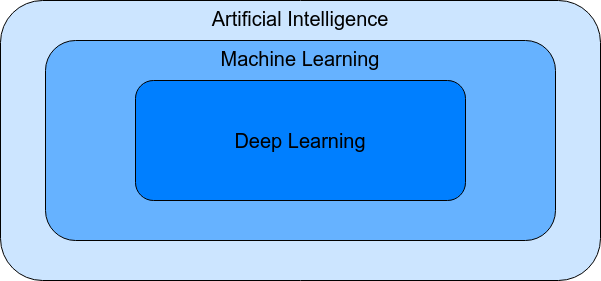
\includegraphics[width=.7\linewidth]{Figures/AI-ML-DL.png}
    \caption{Machine Learning Hierarchy (inspired from Shinde and Shah \cite{shinde2018review})}
    \label{fig:ml-hierarchy}
\end{figure}

Most AI applications follow the process described in the previous paragraph. The set of algorithms that follow this is called machine learning (ML) \cite{el2015machine}. More recently, the most extensive set of algorithms developed is called deep learning (DL) \cite{lecun2015deep,gunning2019xai}, a subset of machine learning algorithms with multiple processing layers to learn abstract data representations.

However, machine and deep learning often find limitations when integrating with edge computing. This condition happens especially when the computing power of the edge application is constrained. Liu et al. \cite{liu2020survey} assert that although many research projects try to reduce this gap, machine, and deep learning often require high computational power and energy consumption. Sze et al. \cite{sze2017hardware} also state that these applications require significant computational power, pushing applications toward the clouds.

\section{Stakeholders}

There are two main stakeholders to the technologies developed in this context. The first stakeholders are professors, students, practitioners, and ecology researchers. The technologies within this context were created aiming for canopy studies and entomology needs. These appliances are usually driven towards environmental perception. Figure \ref{fig:stakeholder-eco} displays some applications developed for these stakeholders.

\begin{figure}[h!]
    \centering
    \includegraphics[width = \linewidth]{Figures/stakeholder-eco.png}
    \caption{Examples of applications developed towards the first stakeholders. These solutions include automatic ant-counting using CNNs, leaf disease detection, and leaf shape estimation.}
    \label{fig:stakeholder-eco}
\end{figure}

The second stakeholders are researchers, physiologists, medical practitioners, patients, and people who require health monitoring appliances. These technologies aim to monitor the users' health conditions and their activities. These applications usually focus on perceiving the users' activities and conditions. Figure \ref{fig:stakeholder-health} displays some applications developed for the second group of stakeholders.

\begin{figure}[h!]
    \centering
    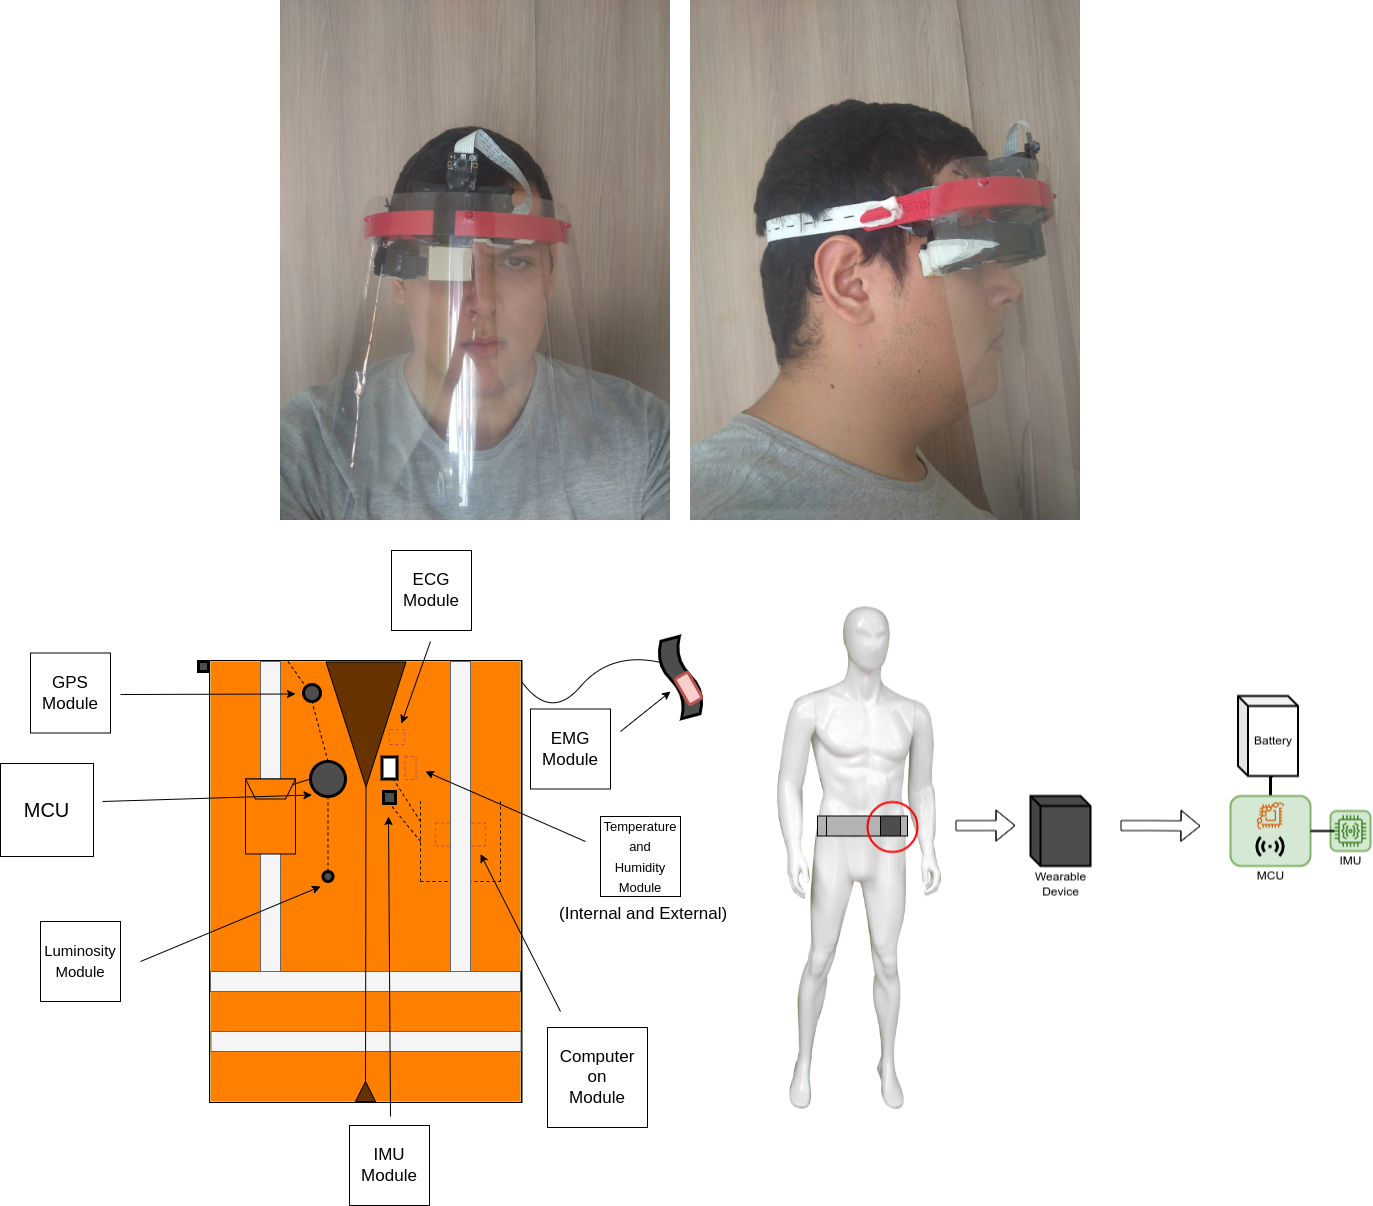
\includegraphics[width = \linewidth]{Figures/stakeholder-health.png}
    \caption{Examples of applications developed towards the second stakeholders. These solutions include health monitoring using a faceshield, a multi-sensored smart vest for industrial applications, and a human activity recognition (HAR) monitor.}
    \label{fig:stakeholder-health}
\end{figure}

\section{Objectives}

In this work, we focus on understanding how to mesh the concepts of edge computing, wearable computing, and AI to create a novel concept within Cyber-Physical Systems. A relatively novel concept named Edge AI works as a baseline for starting this establishment. Therefore, the main objective of this work is:

\begin{itemize}
    \item Establish the concept of Wearable Edge AI and its design process to create cyber-physical applications.
\end{itemize}

We also contemplate a set of specific objectives withing this context. They are:

\begin{itemize}
    \item Propose a novel taxonomy to describe the modalities of Edge AI; 
    \item Develop a set of cyber-physical applications aiming ecological studies;
    \item Develop a set of cyber-physical applications aiming healthcare and human-activity recognition; 
\end{itemize}

\section{Text Organization}

This text is organized into six chapters. In this first chapter, we introduce the subject of the study, motivation, stakeholders, objectives, and contributions. Chapter \ref{chap:establishing} reviews the Edge AI concept and establishes a taxonomy to describe it. Chapter \ref{chap:wearable-edge-ai} displays how we evolved the concept of Wearable Edge AI and defined its design patterns. Chapter \ref{chap:ecology} discusses the applications developed aiming at the ecology stakeholders. Chapter \ref{chap:healthcare} discusses the applications developed aiming at healthcare stakeholders. Finally, we discuss the learned lessons, conclusions, and final remarks in Chapter \ref{chap:conclusions}. 

\section{Contributions}

Within this work's context, we have published the following articles, with a total of 28 citations according to the Google Scholar metrics:

\begin{itemize}
    \item An Automatic Ant Counting and Distribution Estimation System Using Convolutional Neural Networks \cite{Silva2023iceis};
    \item Designing a Multiple-User Wearable Edge AI system towards Human Activity Recognition (2022 XII Brazilian Symposium on Computing Systems Engineering (SBESC)) \cite{silva2022designing};
    \item Edge Computing Smart Healthcare Cooperative Architecture for COVID-19 Medical Facilities (IEEE Latin America Transactions 2022) \cite{silva2022edge};
    \begin{itemize}
        \item 1 citation (Google Scholar);
    \end{itemize}
    \item Bringing Deep Learning to the Fields and Forests: Leaf Reconstruction and Shape Estimation (SN Computer Science, 2022) \cite{silva2022bringing}; 
    \item Wearable Edge AI applications for Ecological Environments (Sensors, 2021) \cite{silva2021wearable};
    \begin{itemize}
        \item 7 citations (Google Scholar);
    \end{itemize}
    \item An Improved Deep Learning Application for Leaf Shape Reconstruction and Damage Estimation (Proceedings of the 23rd International Conference on Enterprise Information Systems - Volume 1: ICEIS, 2021) \cite{iceis21leaf}
    \begin{itemize}
        \item 4 citations (Google Scholar);
        \item Best Student Paper Award in the Area of Artificial Intelligence and Decision Support Systems;
    \end{itemize}
    \item Faceshield HUD: Extended Usage of Wearable Computing on the COVID-19 Frontline (Proceedings of the 23rd International Conference on Enterprise Information Systems - Volume 1: ICEIS, 2021) \cite{iceis21faceshield};
    \begin{itemize}
        \item 1 citation (Google Scholar);
    \end{itemize}
    \item IDiSSC: Edge-computing-based Intelligent Diagnosis Support System for Citrus Inspection (Proceedings of the 23rd International Conference on Enterprise Information Systems - Volume 1: ICEIS, 2021) \cite{iceis21orange};
    \begin{itemize}
        \item 4 citations (Google Scholar);
    \end{itemize}
    \item Leaf shape reconstruction and damage estimation using a U-net-based conditional GAN (Proceedings of the 36th Annual ACM Symposium on Applied Computing - SAC'21, 2021) \cite{silva2021leaf};
    \item Constraints and Challenges in Designing Applications for Industry 4.0: A Functional Approach (Proceedings of the 22nd International Conference on Enterprise Information Systems - Volume 1: ICEIS, 2020) \cite{iceis20robotics};
    \begin{itemize}
        \item 1 citation (Google Scholar);
    \end{itemize}
    \item Field Research Cooperative Wearable Systems: Challenges in Requirements, Design and Validation (Sensors, 2019) \cite{silva2019field};
    \begin{itemize}
        \item 10 citations (Google Scholar);
    \end{itemize}
\end{itemize}

In this period, I have also collaborated with these works with relevant contributions to this topic's knowledge, with 20 more citations:

\begin{itemize}
    \item Towards a mobile system with a new wearable device and an AI application for walking and running activities (Anais do L Semin{\'a}rio Integrado de Software e Hardware, 2023) \cite{alvim2023towards};
    \item A Mobile Robot Based on Edge AI (Anais do L Semin{\'a}rio Integrado de Software e Hardware, 2023) \cite{santos2023mobile};
    \item Towards Autonomous Mobile Inspection Robots Using Edge {AI} (Proceedings of the 25th International Conference on Enterprise Information Systems - Volume 1: ICEIS, 2023) \cite{Santos2023};
    \item Towards a Novel Edge AI System for Particle Size Detection in Mineral Processing Plants (Proceedings of the 25th International Conference on Enterprise Information Systems - Volume 1: ICEIS, 2023) \cite{Cardoso2023};
    \item Blockchain-Based Smart Contract and Edge AI Applied in a Multirobot System: An Approach (IEEE Robotics and Automation Magazine, 2023) \cite{garrocho2023blockchain};
    \item Using Mobile Edge AI to Detect and Map Diseases in Citrus Orchards (Sensors, 2023) \cite{da2023using};
    \begin{itemize}
        \item 2 citations (Google Scholar);
    \end{itemize}
    \item Towards novel smart wearable sensors to classify subject-specific human walking activities (Anais Estendidos do XII Simp{\'o}sio Brasileiro de Engenharia de Sistemas Computacionais) \cite{da2022towards2};
    \item A novel intelligent mobile application using human-centered AR: A case study in orange inspection (Anais Estendidos do XXI Simp{\'o}sio Brasileiro de Fatores Humanos em Sistemas Computacionais) \cite{da2022novel};
    \begin{itemize}
        \item 1 citation (Google Scholar);
    \end{itemize}
    \item Enabling Digital Twins in Industry 4.0 \cite{vitor2022enabling};
    \begin{itemize}
        \item 3 citations (Google Scholar);
    \end{itemize}
    \item Edge Deep Learning Towards the Metallurgical Industry: Improving the Hybrid Pelletized Sinter (HPS) Process \cite{de2022edge};
    \begin{itemize}
        \item 1 citation (Google Scholar);
    \end{itemize}
    \item Towards a novel wearable solution for citrus inspection using Edge AI (2022 IEEE 46th Annual Computers, Software, and Applications Conference (COMPSAC)) \cite{da2022towards};
    \begin{itemize}
        \item 1 citation (Google Scholar);
    \end{itemize}
    \item Applying Edge AI towards Deep-learning-based Monocular Visual Odometry Model for Mobile Robotics (Proceedings of the 24th International Conference on Enterprise Information Systems - Volume 1: ICEIS, 2022) \cite{de2022applying};
    \begin{itemize}
        \item 2 citations (Google Scholar);
    \end{itemize}
    \item Mask R-CNN Applied to Quasi-particle Segmentation from the Hybrid Pelletized Sinter (HPS) Process (Proceedings of the 17th International Joint Conference on Computer Vision, Imaging and Computer Graphics Theory and Applications (VISIGRAPP 2022) - Volume 4: VISAPP) \cite{visapp22hps};
    \item Deep Learning Approach at the Edge to Detect Iron Ore Type (Sensors, 2022) \cite{klippel2022deep};
    \begin{itemize}
        \item 1 citation (Google Scholar);
    \end{itemize}
    \item Deep-Learning-Based Embedded ADAS System (Proceedings of the XI Brazilian Symposium on Computing Systems Engineering (SBESC)) \cite{de2021deep};
    \item Deep-Learning-Based Visual Odometry Models for Mobile Robotics (Proceedings of the XI Brazilian Symposium on Computing Systems Engineering (SBESC)) \cite{de2021deep2};
    \begin{itemize}
        \item 2 citations (Google Scholar);
    \end{itemize}
    \item Synchronous and Asynchronous Requirements for Digital Twins Applications in Industry 4.0 (Proceedings of the 23rd International Conference on Enterprise Information Systems - Volume 1: ICEIS, 2021) \cite{iceis21dt};
    \begin{itemize}
        \item 4 citations (Google Scholar);
    \end{itemize}
    \item Edge Deep Learning Applied to Granulometric Analysis on Quasi-particles from the Hybrid Pelletized Sinter (HPS) Process (Proceedings of the 23rd International Conference on Enterprise Information Systems - Volume 1: ICEIS, 2021) \cite{iceis21hps};
    \begin{itemize}
        \item 3 citations (Google Scholar);
    \end{itemize}
\end{itemize}

We have also deposited a patent request, with its text already in public domain:

\begin{itemize}
    \item ESCUDO FACIAL PARA PROTEÇÃO CONTRA O COVID-19 E DOENÇAS INFECCIOSAS COM MONITOR PORTÁTIL PARA MONITORAMENTO DA SAÚDE DO USUÁRIO E VARIÁVEIS DO AMBIENTE. 2022, Brazil. Registration number: BR1020220014477, INPI - Instituto Nacional da Propriedade Industrial, Brazil.
\end{itemize}

Our total contributions add up to 29 research papers and a deposited patent request, with 48 citations up to this date. We also have two more papers invited to become book chapters. 


\cleardoublepage